\documentclass[a4paper]{article}   	% use "amsart" instead of "article" for AMSLaTeX format
\usepackage{geometry}                		% See geometry.pdf to learn the layout options. There are lots.
%\geometry{left=1.5cm,right=1.5cm,top=1.5cm,bottom=1.5cm}                   		
\usepackage{graphicx,subcaption}					
\usepackage{amssymb}
\usepackage{indentfirst}
\usepackage{amsmath}
\usepackage{amsthm}
\usepackage{bm}
\usepackage{lineno}
\usepackage{setspace}
\usepackage{booktabs,multirow}
\usepackage{authblk}
\usepackage{todonotes}
\usepackage{tikz}
\usepackage{float}
\usepackage[tracking=true]{microtype}
\usetikzlibrary{shapes.geometric, arrows}
\usepackage[title]{appendix}

\usepackage{xcolor}
\newcommand\mynotes[1]{\texttt{\textcolor{orange}{#1}}}
%\renewcommand{\thesubsection}{\Alph{subsection}}

\newtheorem{theorem}{Theorem}
\newtheorem{lemma}[theorem]{Lemma}
\newtheorem{corollary}[theorem]{Corollary}
\newcommand{\E}{\mathrm{E}}
\newcommand{\D}{\mathcal{MD}}
\newcommand{\Var}{\mathrm{Var}}
\newcommand{\Cov}{\mathrm{Cov}}
\newcommand{\Corr}{\mathrm{Corr}}
\newcommand{\tr}{\mathrm{tr}}
\newcommand{\R}{\texttt{R}}
\newcommand{\asreml}{\texttt{ASReml-R}}
\newcommand{\Matern}{Mat\'ern }
\newcommand{\N}{\mathcal{N}}
\newcommand{\AR}{\mathrm{AR1}}
\RequirePackage[colorlinks,citecolor=blue,urlcolor=blue]{hyperref}
\tikzstyle{startstop} = [rectangle, rounded corners, minimum width=3cm, minimum height=1cm,text centered, draw=black, fill=red!30]
\tikzstyle{io} = [trapezium, trapezium left angle=70, trapezium right angle=110, minimum width=0.5cm, minimum height=1cm, text centered, draw=black, fill=blue!30]
\tikzstyle{process} = [rectangle, minimum width=3cm, minimum height=1cm, text centered, draw=black, fill=orange!30]
% \tikzstyle{decision} = [diamond, minimum width=3cm, minimum height=1cm, text centered, draw=black, fill=green!30]
\tikzstyle{decision} = [rectangle, rounded corners, minimum width=3cm, minimum height=1cm,text centered, draw=black, fill=green!30]
\tikzstyle{arrow} = [thick,->,>=stealth]

\usepackage[url=false, isbn=false, eprint=false, backref=false, style= authoryear, backend=bibtex,uniquename=init, maxcitenames=2, giveninits=true, maxbibnames=100]{biblatex}  %%% backend=biber
\DeclareNameAlias{sortname}{family-given} %%% last-first
\addbibresource{BayesOFE.bib}

\renewcommand{\topfraction}{.9}
\renewcommand{\bottomfraction}{.9}
\renewcommand{\textfraction}{.05}
\newcommand{\qtitle}[1]{\textit{\textbf{\textcolor{blue}{#1}}}}
\newcommand{\revision}[1]{\textcolor{red}{#1}}
\newcommand{\reviewer}[1]{\textcolor{blue}{\textit{#1}}}




%\title{Statistical and Economic Analysis of Large Strip Trials in Comparative Experiments} %% Maybe move "On-farm" to keywords

\title{Revision and Response to Reviewers' Comments \\ 
\large on the manuscript (FIELD-D-23-02059R1) \\ Optimal design for on-farm strip trials --- systematic or randomised?}

\author[1,*]{Zhanglong Cao}
\author[1]{Jordan Brown}
\author[1]{Mark Gibberd}
\author[1]{Julia Easton}
\author[1,2]{Suman Rakshit}


\affil[1]{Curtin Biometry and Agricultural Data Analytics, Centre for Crop and Disease Management, Curtin University, Perth, Australia}
\affil[2]{School of Electrical Engineering, Computing and Mathematical Sciences, Curtin University, Perth, Australia}

\affil[*]{Corresponding author: Zhanglong Cao, zhanglong.cao@curtin.edu.au}

\date{}	

\begin{document}
\linenumbers

\maketitle

The authors thank the Associate Editor and Reviewers for their helpful comments and valuable suggestions. All comments/recommendations are addressed below, where each reviewer's comment is presented in \textcolor{blue}{\textbf{blue text}} and each response is given in \textcolor{black}{\textbf{black text}}. As part of this revision process, the newly added materials in the revised draft of the paper are presented using \revision{\textbf{red text}}.




\section*{Reviewer 1 writes:}

\reviewer{This paper compares systematic to randomized designs for on-farm field experimentation. The objective the authors are having in mind is the estimation of spatially varying response functions. The authors find that the systematic design yields more accurate predictions, as anticipated by the authors and some cited references.}

\reviewer{1. My main suggestion is that the authors could also use the exact same simulation to evaluate performance of another objective: Estimation of the marginal regression function, given by the fixed effects b. Randomization theory would be expected to ensure that the randomized design yields unbiased estimates and also yield valid F- and t-tests for treatment effects. It would be very interesting to see how the systematic design fares in comparison when this is the specific purpose of analysis. Of course, as global estimation is the objective in this case, GWR would need to be replaced by classical regression analysis, perhaps just for the model used for simulating the data. Simulating a suitable null hypothesis may also be useful. The linear model could provide a suitable null model for the quadratic as an alternative. Depending on the outcome, such an extension of the simulation would also further accentuate the general conclusion, and potentially enforce the message that a systematic design may be more suitable for local estimation, whereas a randomized design may be preferable for global estimation.}


Thank you for your insightful suggestion. We agree that evaluating the performance of the estimation of the marginal regression function, given by the fixed effects $b$, could provide additional valuable insights. Those are some current research topics that we are working on.  

The difficulty is how to analyse the global effects and what models are appropriate for the topic. \textcite{Stefanova2023Statistical} proposed an approach for comparing the treatments/varieties of a large strip OFE trial by partitioning the entire paddock into smaller regions, named pseudo-environment, then used a MET-like approach to predict the best treatments of each pseudo-environment and the entire paddock. 

We would like to extend our simulation from continuous variables, such as nitrogen rate, to discrete variables, such as varieties, and incorporate \textcite{Stefanova2023Statistical}'s approach to the data to test the performance of systematic designs and randomised designs. The difficulties are how to generate these simulated data robustly,  how to automatically apply the approach to the simulated data in a few iterations, and subsequently to compare the estimated values with the true values.

In the meantime, we are investigating the GAM model, the additive model, with incorporating the spline term to accommodate the spatial variation of OFE. Hopefully, we will achieve nice results for publication. 


\reviewer{2. My major questions are these (see line 156): For the randomized allocation, was a new randomization generated in each simulation run? Or was the same randomization used in each run. Regarding the systematic design, how was the systematic order determined? Was this the same in each simulation run, and was this equal to that shown in Figure 1? Or was a new systematic order chosen in each run. More importantly, what can be said about the optimal systematic order for the purpose of map estimation? How can this optimum be found? How can optimality be defined? It may well be that the authors do not have an answer to this question. However, the question is relevant, and it is worth at least mentioning in the discussion. At any rate, the choice of systematic order the authors made needs to be explained and justified.}

We appreciate the reviewer for pointing out this crucial confusion in this manuscript. It is not clearly explained in the first draft. We have revised the manuscript by the following amendments: 



We added one more subsection \revision{2.3 Performance evaluation} to describe the evaluation of an optimal design: 

\revision{To compare the performances of randomised and systematic designs in terms of accurate estimation of the model coefficients using GWR, we use the mean squared errors (MSE) corresponding to all coefficient estimates. The MSE for a coefficient was computed by first taking the differences between the true coefficient, specified in model (3), and the spatially varying estimates of that coefficient produced by GWR (8), and then averaging these squared differences across all the grid points. The lower the MSE, the better the design’s performance.}



At the beginning of section 4, we rewrote the paragraph that: 

\revision{In this section, we assess the performances of randomised and systematic designs in terms of their utility to accurately estimate the model parameters for both linear and quadratic response models. To this end, we perform 100 simulations of each of the 24 scenarios, described in the previous section. In each simulation, we first generated the coefficients for all grids and then applied the treatment in each grid to calculate the yield value using the model coefficients. For the treatments in all grids, we randomly picked an order of treatments for a single replicate and repeated this sequence across all other replicates to construct a systematic design. For a randomised design, all replicates have different orders of the treatments.}


\reviewer{3. In the Methods section, the subheadings could be reconsidered. Perhaps they can be reworded to clarify the purpose of each model. Which model is used for simulating the data and which model is used for analysing the simulated data?}

Thank you for the comment. I have merged the subsections 2.1 and 2.2 to make a clear explanation of the model, and revised the subsection titles to: \revision{2.1 Hierarchical model for generating simulated data} and \revision{2.2 Fitting geographically weighted regression to simulated data}. Additionally, we have added one more subsection that \revision{2.3 Performance evaluation} to explain how to evaluate the performance. 


\reviewer{4. At the start of Section 3, the authors state an advantage of data simulated from a parametric model. Are there any disadvantages, and what alternatives could be considered? Perhaps this is also a point for the discussion.}

Thank you for your insightful comment. It is right, while data simulated from a parametric model does have its advantages, it also has certain limitations. One potential disadvantage is that the results are heavily dependent on the assumptions of the parametric model. If these assumptions do not hold, the simulation results may not accurately reflect the real-world scenario.

So we have revised Section 3, starting with a better description of the data source and why the parameters are chosen at this level. The simulated data aligns with the authentic data from a corn field in Las Rosa. This data has been studied and reported by \textcite{Rakshit2020Novel, Cao2022Bayesian}. The assumption is based on their findings. 



\reviewer{5. Also at the start of Section 3, where factors studied in the simulation are listed (from line 156), it is not immediately obvious, if the description of details of the simulations refers to the data simulation or the analysis of simulated data. Clarification would be useful. At this point, it is also still not clear which model was used for simulating the data and which for analysing the data. This only becomes clearer gradually downstream in the paper. I feel it could be made very clear much earlier in the paper.}

We have revised Section 3 for a better and clearer explanation. 


\reviewer{6. It may help greatly if the statement of the objectives not made in line 190 comes much earlier.}

We have put a new sentence in the introduction section in line 89: \revision{We subsequently evaluate the efficacy of GWR in accurately estimating the spatially varying treatment effects across these scenarios.}


\reviewer{7. The MSE, used for evaluating predictions, should be described in the section on simulation, as it is part of the methods.}

Thank you for the comment. We agree and have added a new sub-section \revision{2.3 Performance evaluation to describe MSE.}.


\reviewer{8. Line 168: Is the 75 for the mid N level a typo? Should this be 70? Why are the levels different from those in Figure 1?}

Thanks for pointing out the discrepancy. We have revised the mistake by updating the labels in the figures and also in the main context: 

\revision{Figure 1: The nitrogen treatments with five levels (0, 35, 70, 105 and 140 kg/ha) randomly (left) and systematically (right) allocated into strips in each replicate block.}

In line 160: \revision{We used five evenly spaced nitrogen rates: 0, 35, 70, 105, and 140 kg/ha.}

\section*{Reviewer 2 writes:}

\reviewer{The paper presents results from a simulation study to compare two experimental designs, a randomized and a systematic. In my opinion, the subject should be of moderate interest to readers of the journal. The paper needs some work to be considered for publication in FCR, assuming that such technical paper is of interest to most readers of the journal. In its current form I believe it is too technical with a lot of statistical jargon. Also the organization and flow of the information needs to be improved. I made some specific comments about my concerns and on how the authors can improve the manuscript.}

\reviewer{The general suggestion is to revise the text without so much statistical jargon or add explanations that will make it easier for agronomists to follow/understand.}

We have revised the main text of the manuscript to enhance its readability and comprehension. Additionally, we have streamlined the statistical model sections for simplicity and clarity.



\reviewer{Specific comments: 1) Line 40. Please define OFE here and not in line 46 and 57}

We have now defined OFE when it first appears in the main text in line 44. The revised version is \revision{On-farm experiment (OFE) enables farmers the flexibility ...}. 


\reviewer{2) Line 71. Constraints in the field.}

Thanks for pointing out the error. We have changed it to \textit{constraints \revision{in} the field.}

\reviewer{3) Lines 73-74. I do not see the value of that sentence.}

We have polished this paragraph. The purpose of this sentence is to introduce that a linear model may not be sufficient in capturing the yield curve. That's why we compared linear and quadratic curve in this study. 


\reviewer{4) Lines 81-83. These are results and do not fit in the introduction.}

We have rewritten this paragraph to better fit the manuscript by:
\revision{In this study, we generate simulated data for several scenarios, where each scenario is constructed by choosing one component at a time from the following four categories: (i) randomised and systematic designs; (ii) linear and quadratic responses; (iii) model coefficients with low and high correlations; and (iv) spatial variance-covariance matrix  among grids given by identity (no spatial trend), AR1 $\bigotimes$ AR1, and Mat\'{e}rn forms. We subsequently evaluate the efficacy of GWR in accurately estimating the spatially varying treatment effects across these scenarios.}

\reviewer{5) Lines 84-89. There is no need to describe the structure of the paper. All papers have introduction, methods, results and discussion. I suggest to use the last paragraph to describe the objectives of the paper and why is important.}

We have removed this paragraph. Instead, we put one more sentence here: 
\revision{The GWR model in this paper is implemented with the \R-package \texttt{GWmodel} \parencite{lu2014gwmodel, Gollini2015GWmodel}.}

\reviewer{6) Lines 91-93. Again there is no need for these three lines.}

We have removed these lines and re-structured this section by merging subsections 2.1 and 2.2, and inserting a new subsection 2.3. The revised subsection titles are: 

\revision{2.1 Hierarchical model for generating simulated data}.
\revision{2.2 Fitting geographically weighted regression to simulated data}.
\revision{2.3 Performance evaluation}.


\reviewer{7) 3 Simulation study. More information is needed here. I suggest starting from describing the simulated experiment. For example, I had to read up to line 160 and again after line 166 to understand that the independent variable of interest would be nitrogen fertilizer with 5 levels.}

We have rewritten the simulation section by reordering the paragraphs and making a clearer explanation. 

\reviewer{8) Line 172. For someone who is not familiar with systematic design, they would have to read up to line 172 and see figure 1 to understand the difference. I suggest describing what a systematic design is early in the introduction so every reader understands what is being compared.}

We firstly in line 39 inserted the sentence \revision{ where treatments are randomly allocated in each replicate} for a randomised design. 

In line 42, we rewrote the sentence as follows: \revision{With the primary aim of obtaining unbiased estimates of global treatment effects, randomised designs, which use a different layout of treatments in each replicate, are routinely used for on-farm strip trials, whereas systematic designs, which use the same layout of treatments in all replicates, are rarely used.}

In line 168, we try to remind the reader by using the following description that \revision{Examples of a randomised design, which uses different orders of treatment in each replicate, and a systematical design, which uses the same order of treatment in all replicates, are presented in Figure 1.}



\reviewer{9) 4.1 Mean squared error. I recommend to put the figures in order. Now after figure 3 we jump to figure 6 and then figure 4 followed by figure 7.}

Thank you for your suggestion. We have organised the figures in order and updated them with enhanced visualisation.

\reviewer{10) For more practical purposes, apart from comparing MSE and coefficients, it would be valuable to see two maps with optimal nitrogen rate side-by-side. One map generated by the randomized design and one generated by the systematic design. I suspect that for practical purposes maps will be very similar.}

It's a good point. From the practical point of view, that's the most interests output for growers. So, we added one more sub-section at the end of section 4: 
\revision{4.3 An example of optimal nitrogen map} with the description of the results and two optimal nitrogen maps. 


\revision{In practice, growers are more interested in the prescription map that tells them where the appropriate nitrogen should be applied on the paddock. With the application of GWR, we can find the local variations in crop needs, allowing for more precise and efficient nitrogen application. Each grid of the paddock receives the optimal amount of fertiliser. Consequently, this leads to improved crop yields, reduced investment cost and high profit.}

\revision{Figure \ref{fig:optNmap} illustrates an example of the optimal Nitrogen rate (kg/ha) map estimated by GWR with a bandwidth of 9 from a randomised design and a systematic design using the same simulated coefficients of a quadratic curve under the assumption of $\AR\otimes\AR$ spatial covariance and low within-grid correlation. The optimal rate is given by $\hat{N} = -\hat{\beta}_1/(2\hat{\beta}_2)$ with constraints between 0 and 140. For the randomised design, GWR failed to estimate the central part of the paddock. On the contrary, the estimated map from the systematic design is more consistent.}

\begin{figure}[H]
	\begin{subfigure}[t]{0.45\textwidth}
		\centering
		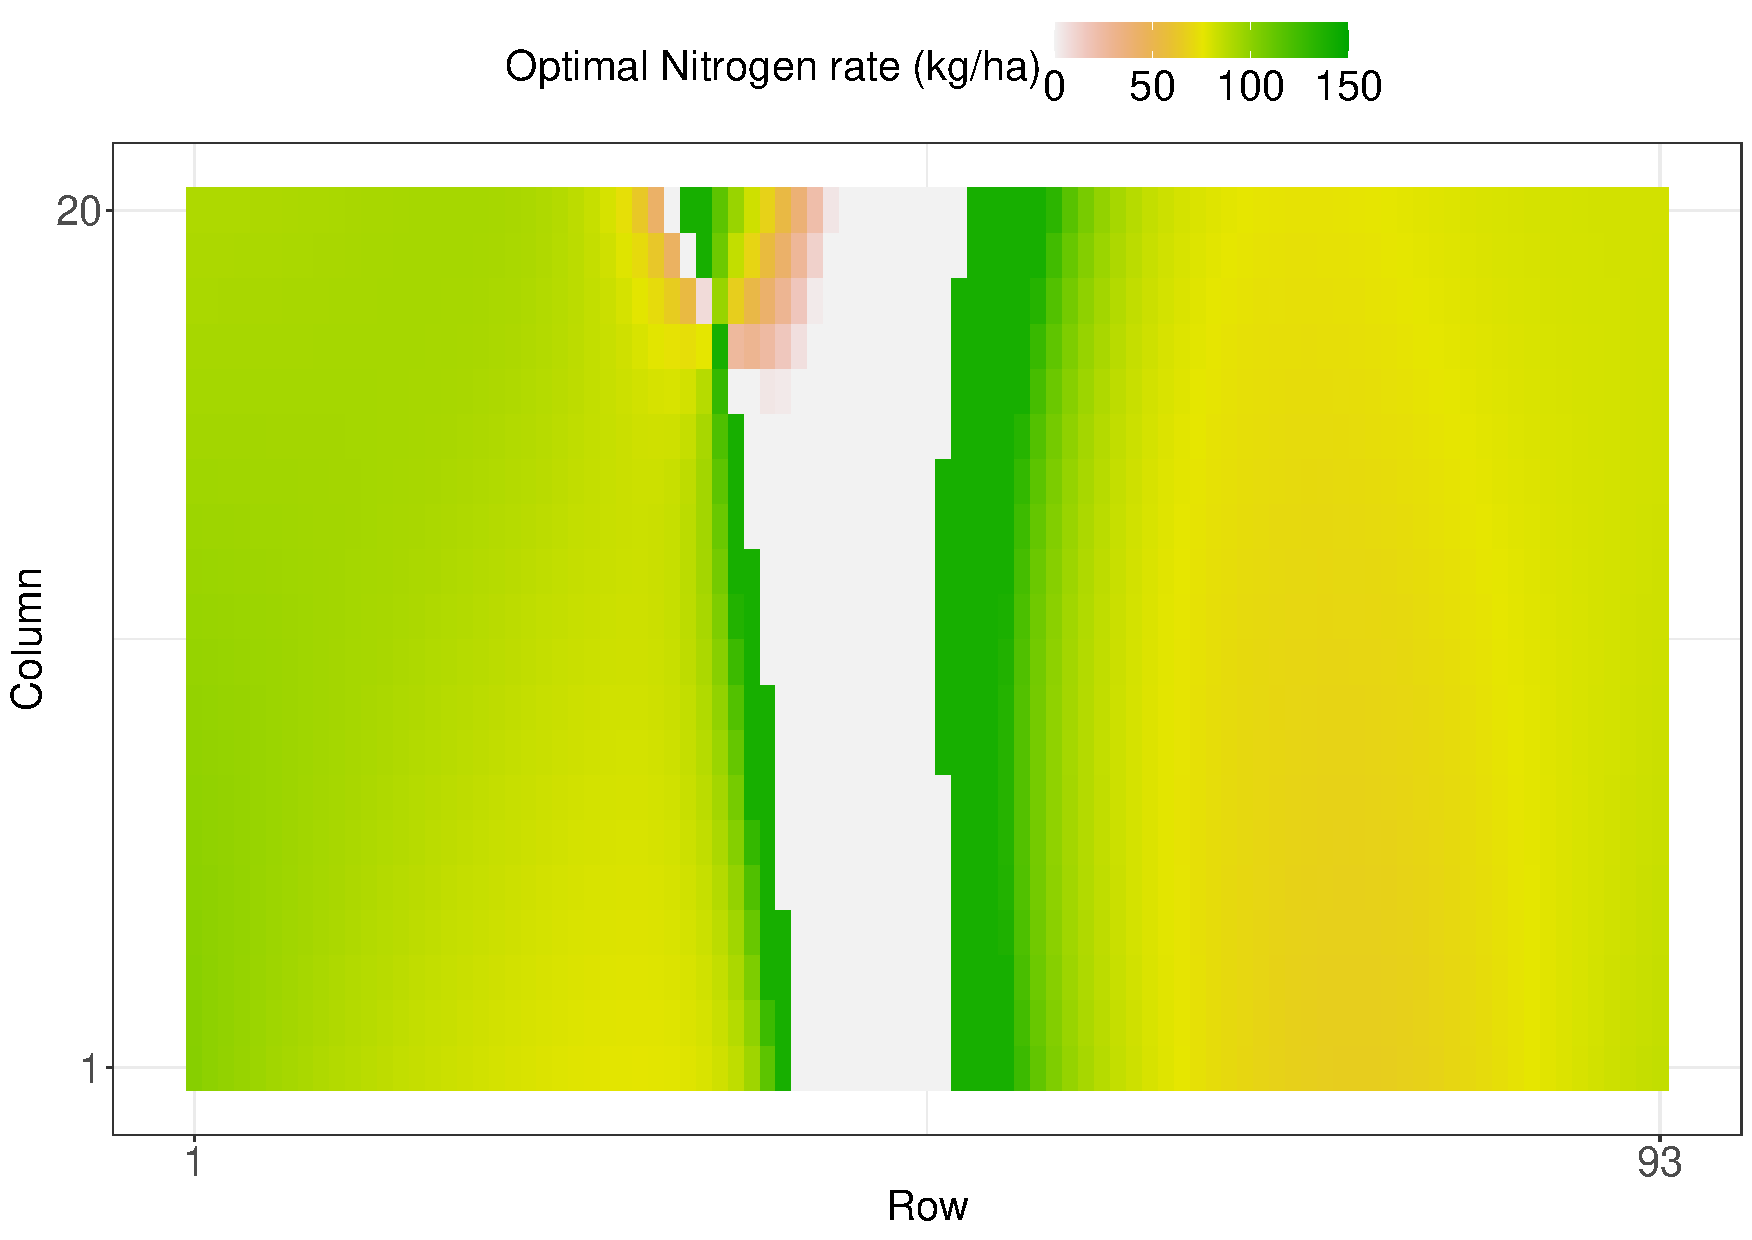
\includegraphics[width=\linewidth]{Expt/optN_syst_AR1B9.pdf}
		%\caption{}
        \end{subfigure}
	\hspace{0.05\textwidth}
	\begin{subfigure}[t]{0.45\textwidth}
		\centering
		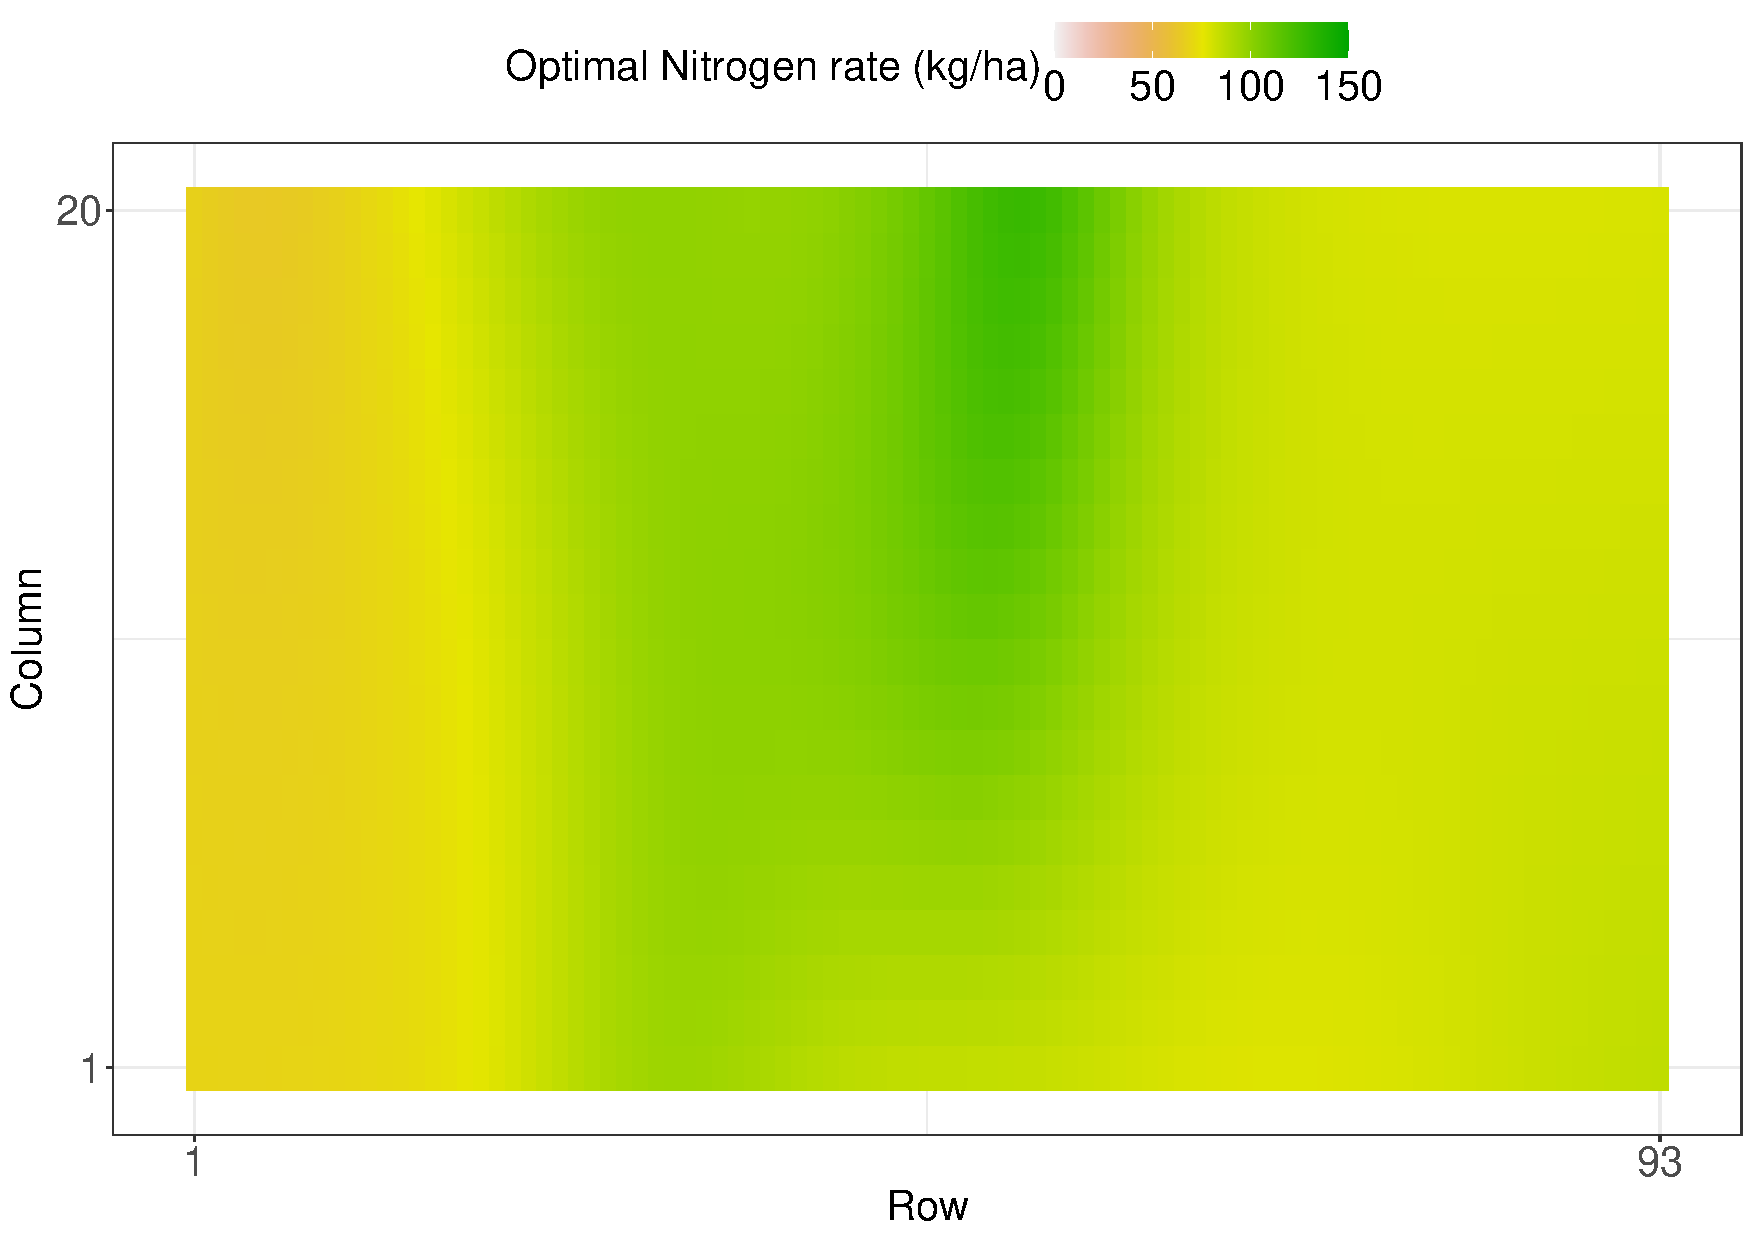
\includegraphics[width=\linewidth]{Expt/optN_rand_AR1B9.pdf}
		%\caption{}
        \end{subfigure}
	\caption{\revision{Optimal Nitrogen rate estimated by GWR from a randomised design (\textit{left}), and a systematic design (\textit{right}).}}\label{fig:optNmap}
\end{figure}

%\printbibliography

\end{document}